
We have good evidence to assume that CPUs can operate much faster on the data already in registers compared to the data in memory. The specifications of the processor and memory speeds alone suggest at least an order of magnitude difference. However, we have learned by now not to make any guesses or assumptions about performance without verifying them through direct measurements. This does not mean that any prior knowledge about the system architecture and any assumptions we can make based on that knowledge are not useful. Such assumptions can be used to guide the experiments and devise the right measurements. We will see in this chapter that the process of discovery by accident can take you only so far and can even lead you into error. The measurements can be correct in and of themselves, but it is often hard to determine what exactly is being measured and what conclusions we can derive from the results.

It would seem that measuring memory access speed should be fairly trivial. All we need is some memory to read from and a way to time the reads, like so:

\begin{lstlisting}[style=styleCXX]
volatile int* p = new int;
*p = 42;
for (auto _ : state) {
	benchmark::DoNotOptimize(*p);
}
delete p;
\end{lstlisting}

This benchmark runs and measures … something. You can expect to get the time of one iteration reported as 0 nanoseconds. This could be the result of an unwanted compiler optimization: if the compiler figures out that the whole program has no observable effects, it may indeed optimize it to nothing. We did take precautions against such an event, though: the memory we read is volatile, and accessing volatile memory is considered an observable effect and cannot be optimized away. Instead, the 0 nanoseconds result is partly a deficiency in the benchmark itself: it suggests that the single read is faster than 1 nanosecond. While this is not quite what we expected based on the memory speed, we can't learn anything, including our own mistakes, from a number we do not know. To fix the measurement aspect of the benchmark, all we have to do is perform multiple reads in one benchmark iteration, like so:

\begin{lstlisting}[style=styleCXX]
volatile int* p = new int;
*p = 42;
for (auto _ : state) {
	benchmark::DoNotOptimize(*p);
	… repeat 32 times …
	benchmark::DoNotOptimize(*p);
}
state.SetItemsProcessed(32*state.iterations());
delete p;
\end{lstlisting}

In this example, we perform 32 reads per iteration. While we could figure out the time of the individual read from the reported iteration time, it is convenient to make the Google Benchmark library do the calculation for us and report the number of reads per second; this is accomplished by setting the number of items processed at the end of the benchmark.

This benchmark should report the iteration time around 5 nanoseconds on a mid-range CPU, confirming that a single read is 1/32 of this time and well below 1 nanosecond (so our guess about the reason why 0 is reported for a single read per iteration is validated). On the other hand, this measured value does not match our expectations for the memory being slow. It is possible that our earlier assumptions about what makes the performance bottleneck are incorrect; it would not be the first time. Or, we could be measuring something other than the memory speed.

\subsubsubsection{4.3.1\hspace{0.2cm}Memory architecture}

To understand how to measure memory performance correctly, we have to learn more about the memory architecture of a modern processor. The most important feature of the memory system, for our purposes, is that it is hierarchical. The CPU does not access the main memory directly but through a hierarchy of caches:

\hspace*{\fill} \\ %插入空行
\begin{center}
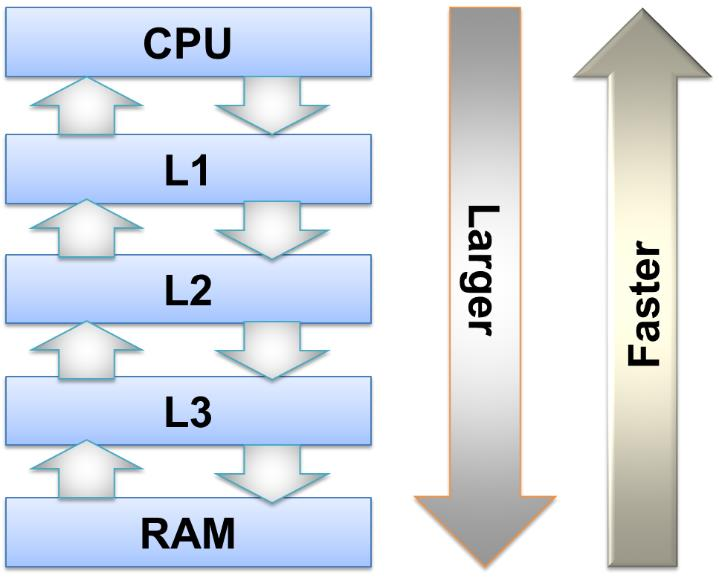
\includegraphics[width=0.9\textwidth]{content/1/chapter4/images/2.jpg}\\
Figure 4.2 – Memory hierarchy diagram
\end{center}

The RAM in Figure 4.2 is the main memory, the DRAM on the motherboard. When the system specifications say that the machine has so many gigabytes of memory, that's the capacity of the DRAM. As you can see, the CPU does not access the main memory directly but instead through several levels of a hierarchy of caches. These caches are also memory circuits, but they are located on the CPU die itself, and they use different technology to store the data: they are all SRAMs of different speeds. The key difference between the DRAM and the SRAM, from our point of view, is that the SRAM is much faster to access, but it draws significantly more power than the DRAM. The speed of the memory access increases as we move closer to the CPU through the memory hierarchy: the level-1 (L1) cache has almost the same access time as the CPU registers, but it uses so much power that we can have only a few kilobytes of such memory, most commonly 32 KB per CPU core. The next level, L2 cache, is larger but slower, the third level (L3) cache is even larger but also slower (and usually shared between multiple cores of a CPU), and the last level of the hierarchy is the main memory itself.

When the CPU reads a data value from the main memory for the first time, the value is propagated through all the cache levels, and a copy of it remains in the cache. When the CPU reads the same value again, it does not need to wait for the value to be fetched from the main memory because a copy of the same value is already available in the fast L1 cache.

As long as the data we want to read fits into the L1 cache, that is all that needs to happen: all the data will be loaded into the cache the first time it's accessed, after that, the CPU only ever needs to access the L1 cache. However, if we try to access a value that is not currently in the cache and the cache is already full, something has to be evicted from the cache to make room for the new value. This process is controlled entirely by the hardware, which has some heuristics to determine which value we are least likely to need again, based on the values we have accessed recently (to the first approximation, the data that wasn't used for the longest time is probably not going to be needed again soon). The next-level caches are larger, but they are used in the same way: as long as the data is in the cache, it is accessed there (the closer to the CPU, the better). Otherwise, it has to be fetched from the next level cache or, for the L3 cache, from the main memory, and, if the cache is full, some other piece of data has to be evicted from the cache (that is, forgotten by the cache, since the original remains in the main memory).

Now we can better understand what we measured earlier: since we were reading the same value over and over, tens of thousands of times, the cost of the initial read was completely lost, and the average read time was that of the L1 cache read. The L1 cache indeed appears to be quite fast, so if your entire data fits into the 32 KB, you do not need to worry about the memory gap. Otherwise, you have to learn how to measure memory performance correctly, so you can draw conclusions that will be applicable to your program.

\subsubsubsection{4.3.2\hspace{0.2cm}Measuring memory and cache speeds}

Now that we understand that the memory speed is more complex than just the time of a single read, we can devise a more appropriate benchmark. We can expect the cache sizes to affect the results significantly, so we have to access data of different sizes, from several kilobytes (fits into the 32 KB L1 cache) to tens of megabytes or more (L3 cache sizes vary but are usually around 8 MB to 12 MB). Since, for large data volumes, the memory system will have to evict the old data from the cache, we can expect the performance to depend on how well that prediction works or, more generally, on the access patterns. Sequential access, such as copying a range of memory, may end up performing very differently than accessing the same range in random order. Finally, the results may depend on the granularity of the memory access: is accessing a 64-bit long value slower than accessing a single char?

A simple benchmark for sequentially reading a large array can look like this:

\begin{lstlisting}[style=styleCXX]
// 01c_cache_sequential_read.C
template <class Word>
void BM_read_seq(benchmark::State& state) {
	const size_t size = state.range(0);
	void* memory = ::malloc(size);
	void* const end = static_cast<char*>(memory) + size;
	volatile Word* const p0 = static_cast<Word*>(memory);
	Word* const p1 = static_cast<Word*>(end);
	for (auto _ : state) {
		for (volatile Word* p = p0; p != p1; ) {
			REPEAT(benchmark::DoNotOptimize(*p++);)
		}
		benchmark::ClobberMemory();
	}
	::free(memory);
	state.SetBytesProcessed(size*state.iterations());
	state.SetItemsProcessed((p1 - p0)*state.iterations());
}
\end{lstlisting}

The benchmark for writing looks very similar, with a one-line change in the main loop:

\begin{lstlisting}[style=styleCXX]
// 01d_cache_sequential_write.C
Word fill = {}; // Default-constructed
for (auto _ : state) {
	for (volatile Word* p = p0; p != p1; ) {
		REPEAT(benchmark::DoNotOptimize(*p++ = fill);)
	}
	benchmark::ClobberMemory();
}
\end{lstlisting}

The value we write into the array should not matter; if you are concerned that zero is somehow special, you can initialize the fill variable with any other value.

The macro REPEAT is used to avoid manually copying the benchmarked code many times. We still want to perform several memory reads per iteration: while avoiding the 0 nanoseconds per iteration report is less critical once we start reporting the number of reads per second, the overhead of the loop itself is non-trivial for a very cheap iteration like ours, so it is better to unroll this loop manually. Our REPEAT macro unrolls the loop 32 times:

\begin{lstlisting}[style=styleCXX]
#define REPEAT2(x) x x
#define REPEAT4(x) REPEAT2(x) REPEAT2(x)
#define REPEAT8(x) REPEAT4(x) REPEAT4(x)
#define REPEAT16(x) REPEAT8(x) REPEAT8(x)
#define REPEAT32(x) REPEAT16(x) REPEAT16(x)
#define REPEAT(x) REPEAT32(x)
\end{lstlisting}

Of course, we have to make sure that the memory size we request is large enough for the 32 values of the Word type and that the total array size is divisible by 32; neither is a significant restriction on our benchmark code.

Speaking of the Word type, this is the first time we used a TEMPLATE benchmark. It is used to generate the benchmarks for several types without copying the code. There is a slight difference in invoking such a benchmark:

\begin{lstlisting}[style=styleCXX]
#define ARGS ->RangeMultiplier(2)->Range(1<<10, 1<<30)
BENCHMARK_TEMPLATE1(BM_read_seq, unsigned int) ARGS;
BENCHMARK_TEMPLATE1(BM_read_seq, unsigned long) ARGS;
\end{lstlisting}

If the CPU supports it, we can read and write the data in even larger chunks, for example, using SSE and AVX instructions to move 16 or 32 bytes at a time on an x86 CPU. In GCC or Clang, there are library headers for these larger types:

\begin{lstlisting}[style=styleCXX]
#include <emmintrin.h>
#include <immintrin.h>
…
BENCHMARK_TEMPLATE1(BM_read_seq, __m128i) ARGS;
BENCHMARK_TEMPLATE1(BM_read_seq, __m256i) ARGS;
\end{lstlisting}

The types \_\_m128i and \_\_m256i are not built into the language (at least not C/C++), but C++ lets us declare new types easily: these are value-type classes (classes that represent a single value), and they have a set of arithmetic operations defined for them, such as addition and multiplication, which the compiler implements using the appropriate SIMD instructions.

The preceding benchmark accesses the memory range sequentially, from the beginning to the end, in order, one word at a time. The size of the memory varies, as specified by the benchmark arguments (in the example, from 1 KB to 1 GB, doubling every time). After the memory range is copied, the benchmark does it again, from the beginning, until enough measurements are accumulated.

More care must be taken when measuring the speed of accessing the memory in random order. The naïve implementation would see us benchmarking the code that looks something like this:

\begin{lstlisting}[style=styleCXX]
benchmark::DoNotOptimize(p[rand() % size]);
\end{lstlisting}

Unfortunately, this benchmark measures the time it takes to call the rand() function: it is so much more computationally expensive than reading a single integer that you'll never notice the cost of the latter. Even the modulo operator \% is significantly more expensive than a single read or write. The only way to get something remotely accurate is to precompute the random indices and store them in another array. Of course, we have to contend with the fact that we're now reading both the index values and the indexed data, so the measured cost is that of two reads (or a read and a write).

The additional code for writing memory in random order can be as follows:

\begin{lstlisting}[style=styleCXX]
// 01b_cache_random_write.C
const size_t N = size/sizeof(Word);
std::vector<int> v_index(N);
for (size_t i = 0; i < N; ++i) v_index[i] = i;
std::random_shuffle(v_index.begin(), v_index.end());
int* const index = v_index.data();
int* const i1 = index + N;
Word fill; memset(&fill, 0x0f, sizeof(fill));
for (auto _ : state) {
	for (const int* ind = index; ind < i1; ) {
		REPEAT(*(p0 + *ind++) = fill;)
	}
	benchmark::ClobberMemory();
}
\end{lstlisting}

Here we use the STL algorithm random\_shuffle to generate a random order of indices (we could have used random numbers instead; it's not exactly the same since some indices would have appeared more than once and others never, but it should not affect the results much). The value we write should not really matter: writing any number takes the same time, but the compiler can sometimes do special optimizations if it can figure out that the code is writing a lot of zeroes, so it's best to avoid that and write something else. Note also that the longer AVX types cannot be initialized with an integer, so we write an arbitrary bit pattern into the writing value using memset().

The benchmark for reading is, of course, very similar, just the inner loop has to change:

\begin{lstlisting}[style=styleCXX]
REPEAT(benchmark::DoNotOptimize(*(p0 + *ind++));)
\end{lstlisting}

We have the benchmarking code that measures mostly the cost of the memory access. The arithmetic operations necessary to advance the indices are unavoidable, but the additions take a single cycle at most, and we have already seen that the CPU can do several at once, so the math is not going to be the bottleneck (and, in any case, any program that accesses memory in an array would have to do the same computations, so this is the access speed that matters in practice). Now let us see the results of our efforts.




























